%%%%%%%%%%%%%%%%%%%%%%%%%%%%%%%%%
\subsection{General}

The end goal of the project is to develop an efficient system for image vectorization. The system would take any image as input and output an SVG representation of the original image. The system is mainly composed of 3 different components.

%%%%%%%%%%%%%%%%%%%%%%%%%%%%%%%%%
\subsection{Sampling}

The sampling process is based on \cite{zhao2013image}. The input image is a regular bitmapped image, such as \cref{fig:arch_original}. The first step is to apply the gradient operator on the image to get the importance matrix, shown in \cref{fig:arch_importance}. This involves pixel-wise convolving with four $3\times 3$ Sobel filters (horizontal, vertical, and two diagonals) and finding the magnitude to determine the magnitude of the gradient, which is interpreted as the local information content or ``importance'' of the area surrounding a given pixel. Next, the importance matrix is thresholded so that only points of high importance are retained, shown in \cref{fig:arch_thresholded}. This is essentially a high-pass filter; low-frequency components of the image are lost. The intuition is that low-frequency elements can be represented with uniformly-colored shapes without much information loss.

Now we perform the sampling to obtain \cref{fig:arch_sampled}. The sampling density at a pixel is a function of the importance of that pixel; a higher importance leads to a higher sampling frequency. This is known as ``blue-noise'' sampling, and allows us to focus more detail on regions of higher information content. After sampling, the image is converted to a triangular mesh by performing the Delaunay triangulation, as shown in \cref{fig:arch_triangulated}.

% TODO: include formula for sampling density and explain it
% TODO: explain method for sampling (poisson disks?)

\begin{figure}[H]
    \centering
    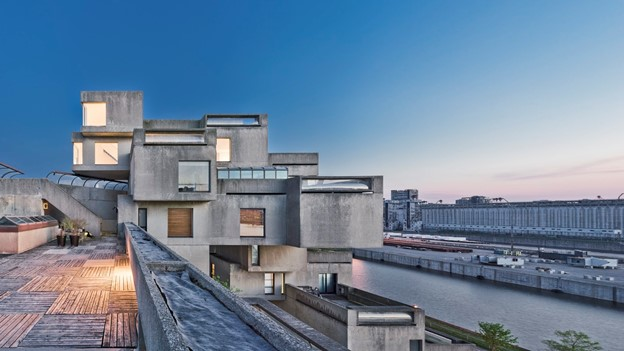
\includegraphics[width=\linewidth]{Figures/vectorization_images/original.jpg}
    \caption{Original image}
    \label{fig:arch_original}
\end{figure}

\begin{figure}[H]
    \centering
    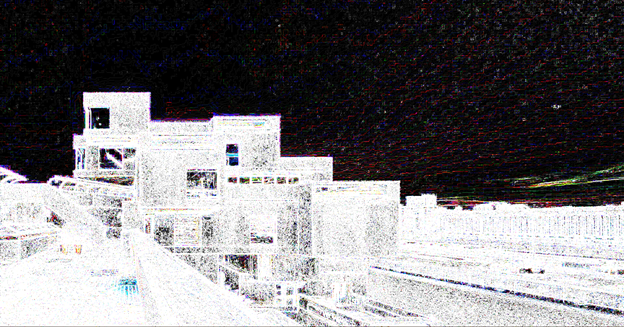
\includegraphics[width=\linewidth]{Figures/vectorization_images/importance.png}
    \caption{Importance function applied to the image}
    \label{fig:arch_importance}
\end{figure}

\begin{figure}[H]
    \centering
    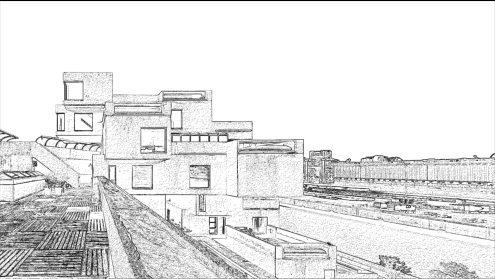
\includegraphics[width=\linewidth]{Figures/vectorization_images/thresholded.png}
    \caption{Thresholded points}
    \label{fig:arch_thresholded}
\end{figure}

\begin{figure}[H]
    \centering
    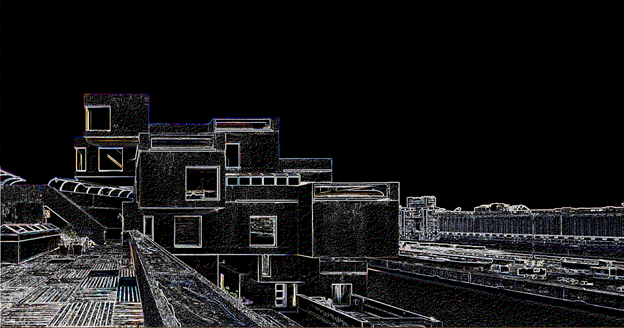
\includegraphics[width=\linewidth]{Figures/vectorization_images/sampled.png}
    \caption{Sampled points}
    \label{fig:arch_sampled}
\end{figure}

\begin{figure}[H]
    \centering
    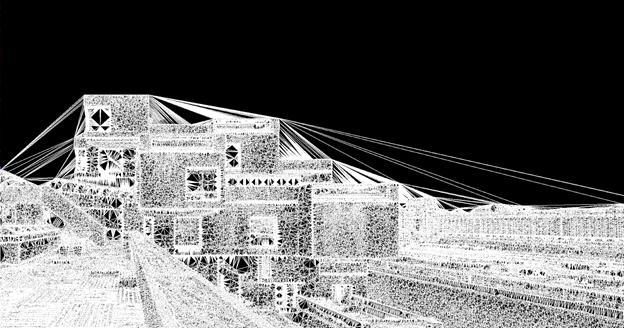
\includegraphics[width=\linewidth]{Figures/vectorization_images/triangulated.png}
    \caption{Triangulated image}
    \label{fig:arch_triangulated}
\end{figure}

%%%%%%%%%%%%%%%%%%%%%%%%%%%%%%%%%
\subsection{Mesh Optimization}

This is a future goal for spring semester and has not been implemented yet.

%%%%%%%%%%%%%%%%%%%%%%%%%%%%%%%%%
\subsection{Triangle Mesh Coloring}

We currently have three methods for determining what color to use for each triangle. The first method takes the mean of the RGB values at the three points of the triangle. The second method randomly samples a set number of integer points inside of the triangle and takes the mean of the RGB values of those points. The third method takes the mean of the RGB values at every integer point in the triangle. We note that the third method approximates the triangle, so it may sample integer points outside of the triangle. In addition, the third method utilizes the first method for small triangles, where the number of integer points inside the triangle is less than three.

%%%%%%%%%%%%%%%%%%%%%%%%%%%%%%%%%
\subsection{Writing to SVG}

We convert internal representations of triangles (tuples with 3 pairs, representing the coordinates of each point on the triangle) to an SVG file. We use Python's pycairo library to accomplish this.

In the future, we may also attempt to optimize this, such as by coding redundant information.

%%%%%%%%%%%%%%%%%%%%%%%%%%%%%%%%%
\subsection{Evaluation Metric}

We implemented an evaluation metric based on content loss from \customcite{dumoulin2017learned}. Similar to the methodology used by the authors, We use a pre-trained VGG-19 and strip off the $conv_5$ and fully-connected blocks. It is important to note that the authors used a VGG-16. We use a VGG-19, similar to \customcite{huang2017arbitrary}. In order to get the content loss between two images, we take the Euclidean distance between the outputs of the stripped VGG-19.

% We tested the content loss metric on three images related to style transfer using Generative Adversarial Networks. The images were from \url{https://www.tensorflow.org/tutorials/generative/style_transfer}. 

% \begin{figure}[H]
%     \centering
%     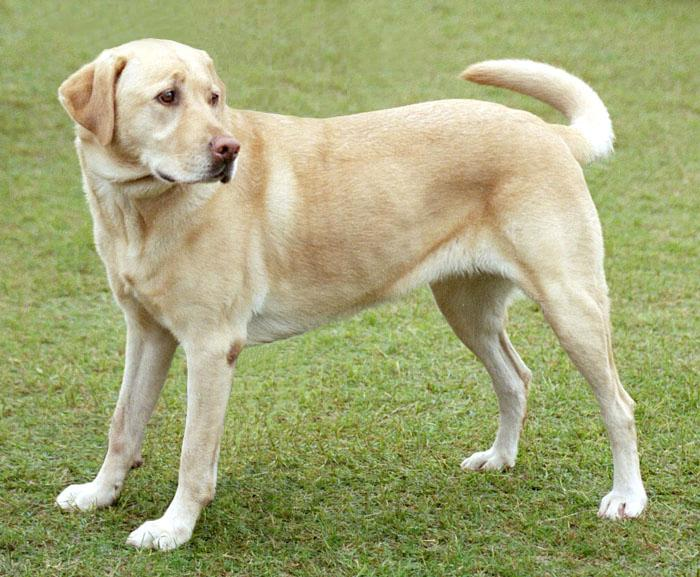
\includegraphics[width=\linewidth]{Figures/content_loss_images/lab1.jpg}
%     \caption{\href{https://commons.wikimedia.org/wiki/File:YellowLabradorLooking_new.jpg}{Yellow Labrador Looking}, from Wikimedia Commons}
%     \label{fig:lab_original}
% \end{figure}

% \begin{figure}[H]
%     \centering
%     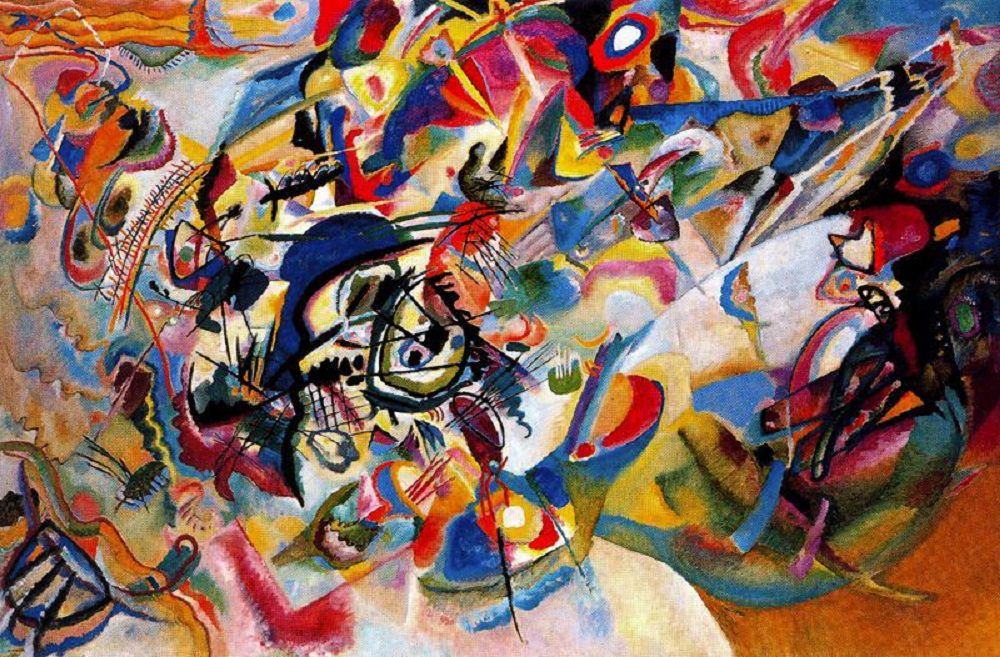
\includegraphics[width=\linewidth]{Figures/content_loss_images/lab2.jpg}
%     \caption{Composition VII by Wassily Kandinsky}
%     \label{fig:lab_style}
% \end{figure}

% \begin{figure}[H]
%     \centering
%     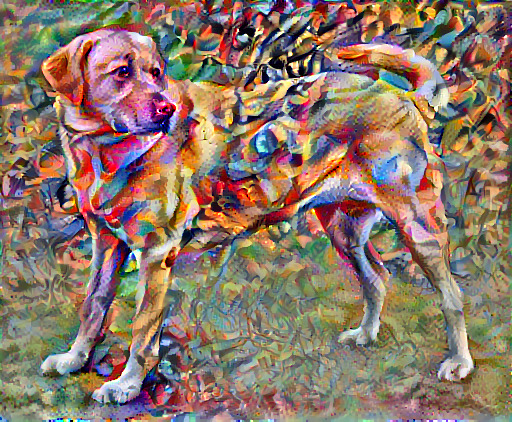
\includegraphics[width=\linewidth]{Figures/content_loss_images/lab3.jpg}
%     \caption{Generated image produced with style transfer}
%     \label{fig:lab_style_transfer}
% \end{figure}

% \cref{fig:lab_style_transfer} is generated using the content from \cref{fig:lab_original} and the style from \cref{fig:lab_style}. We calculated the content loss between all three pairings of the above images. The results are displayed in the table below.

% \begin{table}[H]
%     \centering
%     \begin{tabular}{| c | c | c |}                                             \hline
%         Image 1 & Image 2 & Content Loss                                    \\ \hline
%         \cref{fig:lab_original} & \cref{fig:lab_style_transfer} & 132352.05 \\ \hline
%         \cref{fig:lab_original} & \cref{fig:lab_style} & 190958.28          \\ \hline
%         \cref{fig:lab_style} & \cref{fig:lab_style_transfer} & 190266.86    \\ \hline
%     \end{tabular}
%     \caption{Sample content loss for example images}
%     \label{tab:lab_content_loss}
% \end{table}

% As can be seen in \cref{tab:lab_content_loss}, the lowest content loss is between \cref{fig:lab_original} and \cref{fig:lab_style_transfer}, which is expected. In addition, the content loss between \cref{fig:lab_style} and the other two images is almost the same, which makes sense, because the other two images should have the same content with different style.

% We may want to refine this evaluation metric in the future. The content loss values are extremely large and are difficult to interpret on their own. We may wish to use a baseline image when comparing the results of our project. We would thus compare three images (the original image, the vectorized image, and the baseline image). This baseline image can be arbitrarily selected. The purpose of the baseline image is to provide context to the content loss values. Similar to the above example, we would compare all three pairings of the images. We would want the content loss between the original image and the vectorized image to be the lowest. We would also want the content loss for the other two pairings (with the baseline image) to be relatively similar.

\begin{figure}[H]
    \centering
    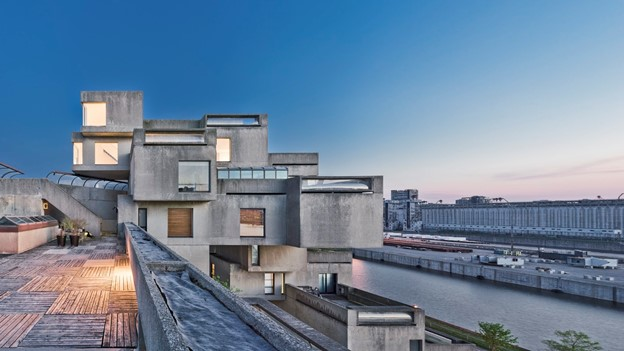
\includegraphics[width=\linewidth]{Figures/vectorization_images/original.jpg}
    \caption{Original image}
    \label{fig:house_original}
\end{figure}

\begin{figure}[H]
    \centering
    \includesvg[width=\linewidth]{Figures/vectorization_images/house_potrace.svg}
    \caption{Vectorized image created with Potrace}
    \label{fig:house_potrace}
\end{figure}

\begin{figure}[H]
    \centering
    \includesvg[width=\linewidth]{Figures/vectorization_images/house_our_method.svg}
    \caption{Vectorized image created with our method}
    \label{fig:house_our_method}
\end{figure}

\begin{table}[H]
    \centering
    \begin{tabular}{| c | c | c |}     \hline
        Method & Content Loss       \\ \hline
        Our Method & 118758.836     \\ \hline
        Potrace & 141575.78         \\ \hline
    \end{tabular}
    \caption{Content loss for vectorizing a sample image with different methods}
    \label{tab:house_content_loss}
\end{table}

As seen in \cref{tab:house_content_loss}, our method produces a significantly lower content loss than Potrace.

%%%%%%%%%%%%%%%%%%%%%%%%%%%%%%%%%
\subsection{Implementation stack}

The current implementation is a mix of Python and C++. The image processing components utilize OpenCV for GPU support and will be multi-threaded. Efficiency of the process is not a concern at this point; we care more about optimizing for the error metric. Future iterations of this project may consider efficiency of implementation.
